\RequirePackage[T1]{fontenc}
\documentclass[journal,10pt]{IEEEtran}
\usepackage{mathptmx}
\usepackage{amsmath,amssymb,booktabs,array,multirow}
\usepackage{graphicx,xcolor}
\usepackage{placeins}
\usepackage{algorithm,algpseudocode}
\usepackage{cite,url}
\usepackage[hidelinks]{hyperref}
\usepackage{tikz}
\usetikzlibrary{arrows.meta,positioning,fit,calc}
\newcommand{\LEAF}{\textsc{LEAF}}
\hyphenation{multi-agent gene-ra-li-za-tion re-pre-sen-ta-tion}
\hypersetup{pdftitle={LEAF: Looped Entity Attention Fusion for Population-Generalizable Multi-Agent Defense},pdfauthor={}}
\begin{document}
\title{LEAF: Looped Entity Attention Fusion for Population-Generalizable Multi-Agent Defense}
\author{Anonymous Authors}
\bstctlcite{leafBibliographyControl}
\maketitle
\markboth{Anonymous Manuscript Submitted for Review}{LEAF: Looped Entity Attention Fusion}
\begin{abstract}
Cooperative target protection requires defenders to interpret threats in the context of nearby teammates and protected assets as their populations change. We propose Looped Entity Attention Fusion (LEAF), a receiver-conditioned relational encoder for cooperative value learning. A shared attention block iteratively updates the entity representations, a query derived from the acting defender reads each intermediate representation, and learned fusion combines these reads before a recurrent decision network. This design couples current-scene contextual processing with intermediate-stage access while retaining temporal memory downstream. In SkyHAD, policies trained with at most ten vehicles per team and three targets are evaluated without retraining on 24 configurations reaching 50 vehicles per team and 12 targets. Across three training seeds, LEAF improves mean reward over REFIL by 0.800, 1.635, and 2.211 in target-count, team-size, and joint extrapolation, respectively. Trained architectural comparisons favor contextual processing before reading and current-state queries with downstream memory. Normal forward records show receiver-specific fusion concentrated on early contextual reads, while evaluations across trained depths characterize scene-dependent refinement. At 50 vehicles per team and two targets, attacker interception increases from 72.27\% to 78.68\%, while the incidence of target damage decreases from 70.56\% to 28.11\%. These results support relational encoding as a practical approach to population transfer in cooperative defense.
\end{abstract}
\noindent\textbf{Note to Practitioners---}
A cooperative protection controller may need to operate with different numbers of defending vehicles, incoming threats, and protected assets. LEAF uses a shared policy that accepts a variable-size set of observed entity states. Each defender builds the current scene context, reads it from its own perspective, and combines it with a recurrent temporal state to choose an action. The controller is trained on small engagements and reused with frozen parameters in larger ones. Evaluation measures both protected-asset reward and friendly-collision mortality, allowing the two operational outcomes to be assessed together. The study uses the planar vehicle model in SkyHAD with public entity-state observations and a reactive attacker. This interface suits simulation-based assessment of cooperative protection strategies and can serve as the policy layer when integrating platform-specific sensing and actuation.
\par
\begin{IEEEkeywords}
Multi-agent reinforcement learning, cooperative control, population generalization, entity attention, target protection.
\end{IEEEkeywords}
\section{Introduction}
\IEEEPARstart{C}{ooperative} target protection requires a team to respond to several threats at once. A defender approaching one attacker must account for the target behind that attacker, nearby teammates, and competing threats elsewhere. As vehicles are intercepted and threats move between targets, the useful relationships change. A controller trained for a small engagement should reuse these relationships when more defenders, attackers, or protected assets enter the scene. This requirement motivates policies that coordinate through entity relationships rather than a fixed population layout.

Entity-based multi-agent reinforcement learning provides a suitable starting point. Shared set encoders accept variable numbers of entities, while attention extracts information for each agent~\cite{zaheer2017deepsets,lee2019settransformer}. REFIL further encourages reusable interactions through randomized entity-wise value factorization~\cite{iqbal2021refil}. The remaining design question concerns the representation supplied to the controller: how should an individual defender interpret an attacker together with its surrounding teammates and targets, and retain the parts of that context that matter for its next action?

We address this question through \emph{receiver-conditioned, multi-stage relational encoding}. A shared attention block repeatedly updates the entity representations within one physical decision. Each update operates on the context produced by the preceding update. A reader conditioned on the defender's own state accesses every intermediate representation, and a learned fusion combines these reads into the decision feature. Context construction and reading form one encoder: the loop develops relations among entities, while the reader expresses those relations from the perspective of the acting defender. Keeping intermediate reads lets the controller use early context alongside later refinements.

This computation has a different role from memory across physical time. An attacker's target assignment is private, although its position and velocity are observed. The policy therefore retains a recurrent state to interpret motion over successive observations. We use the current self state to query the relational encoder and place temporal recurrence downstream. The resulting architecture, \textbf{Looped Entity Attention Fusion (LEAF)}, augments REFIL's feature with the fused relational read and then updates the defender's GRU once. Network parameters are shared across entities, defenders, and processing rounds. Training samples one to four rounds, and the deployed policy uses four.

Our evaluation follows the intended control problem. In SkyHAD~\cite{skyhad2026}, policies learn with at most ten vehicles per team and three targets, then execute with frozen parameters on 24 configurations reaching 50 vehicles per team and 12 targets. We compare LEAF with REFIL, QMIX-Atten, DCG, SPECTra, ALMA, and a rule-based controller. Reward is the negative of accumulated target damage. LEAF attains the highest group mean reward among these methods in the in-distribution, target-count, team-size, and joint-extrapolation groups. Its gains over REFIL are accompanied by fewer friendly-collision deaths and more attacker interceptions.

The experiments connect this outcome to the representation design. Trained comparisons examine reading before and after contextual processing, placing memory in the reader, and retaining the REFIL host. Execution at the four depths used in training characterizes how refinement affects the frozen policy. Normal forward records then show which intermediate reads supply its decisions, while common-scene trajectories connect interception behavior to target protection. The contributions are:
\begin{enumerate}
\item A receiver-conditioned relational encoder that couples shared iterative entity updates with fusion of intermediate reads, integrated with recurrent cooperative value learning.
\item A population-transfer evaluation covering changes in vehicle and target counts, with learning curves, two operational metrics, and trained architectural comparisons across three training seeds.
\item An empirical account of the controller's operation that connects contextual processing and intermediate-read use to interception and target-protection outcomes.
\end{enumerate}

\section{Related Work}
\subsection{Target Defense and Reach--Avoid Games}
Cooperative target defense couples interception with protection: defenders must account for both approaching adversaries and the assets they threaten. Differential-game approaches characterize this interaction through geometry, winning regions, and feedback strategies. Garcia et al. derive state-feedback optimal strategies for active defense~\cite{garcia2019activedefense}. For larger teams, Chen et al. combine pairwise reach--avoid outcomes through matching~\cite{chen2017reachavoid}, while Yan et al. use analytical barriers to determine coalition capabilities and formulate task assignment in convex domains~\cite{yan2020barriers}. Matching-based strategies also address three-dimensional heterogeneous teams, combining capture subgames with repeated allocation~\cite{yan2022matching}.

Perimeter defense emphasizes the team outcome when multiple intruders approach a protected region. Shishika et al. develop a decomposition and assignment strategy that explicitly accommodates cooperative defense~\cite{shishika2020perimeter}. This literature establishes that interception opportunities depend on the joint arrangement of defenders and intruders, making the distribution of team effort central to protection. The analytical methods obtain guarantees under their specified dynamics and geometry. Our setting evaluates a learned maneuver policy using cumulative damage to stationary targets, with the same policy deployed across different vehicle and target populations. These changes alter the interactions that the policy must represent and the allocation of effort implicit in its actions.

\subsection{Task Allocation and Cooperative Learning}
Task allocation provides an explicit way to organize multi-robot effort. Gerkey and Matari\'{c} give a formal taxonomy of allocation problems~\cite{gerkey2004allocation}, and consensus-based decentralized auctions combine local bidding with conflict resolution~\cite{choi2009auction}. Cooperative tasks can require robot coalitions: Deng et al. develop distributed auctions for two-robot coalitions, including time-varying assignments and multiplayer reach--avoid applications~\cite{deng2024coalitions}. Miele et al. integrate distributed allocation with safe movement, connectivity maintenance, and deadlock handling~\cite{miele2025coordination}. These approaches expose assignment and motion coordination as coupled decisions.

Learning offers complementary ways to couple these decisions. Centralized training with decentralized execution supports cooperation through multi-agent actor--critic methods and team-reward policy optimization~\cite{lowe2017maddpg,yu2022mappo}. Coach-player learning additionally addresses changing team composition through individual strategies supplied by a coordinating coach~\cite{liu2021copa}. Cooperative distributional reinforcement learning has been applied to dynamic multi-ship weapon--target assignment with attention and delayed rewards~\cite{peng2025wta}. In automation settings, hierarchical learning combines allocation and planning for uncertain swarm confrontation~\cite{wu2025swarm}, and observer-assisted multi-agent learning addresses pursuit--evasion under unknown uncertainties~\cite{liu2025observer}. Closely related to target protection, Li et al. organize learning into intention recognition, target allocation, and path execution~\cite{li2025targetdefense}. Their hierarchy uses differential-game information during allocation training. LEAF instead learns defender action values through a common entity representation, allowing coordination to emerge through maneuver decisions without a separate assignment output. Its contribution concerns the joint relational encoder that supplies these values; the cooperative value-learning objective remains based on REFIL.

\subsection{Entity Representation and Multi-Stage Relational Encoding}
Variable-size entity representations are established tools for cooperative learning. Deep Sets and Set Transformers encode unordered inputs~\cite{zaheer2017deepsets,lee2019settransformer}, while swarm reinforcement learning uses mean embeddings to represent changing neighborhoods~\cite{huttenrauch2019swarm}. Value decomposition, monotonic mixing, and coordination graphs connect agent utilities with team objectives~\cite{sunehag2018vdn,rashid2018qmix,boehmer2020dcg}. REFIL combines entity attention with randomized entity partitions and an auxiliary factorized value objective~\cite{iqbal2021refil}. UPDeT and TransfQMix use transformers in cooperative policies and mixing networks~\cite{hu2021updet,transfqmix2023}; SPECTra emphasizes permutation-consistent scalable networks~\cite{park2026spectra}, and ALMA addresses composite tasks through hierarchical learning~\cite{iqbal2022alma}. Spatial aggregation and temporal recurrence have also been combined for perimeter defense: GR-MAPPO uses GraphSAGE and a GRU and evaluates cross-scale transfer~\cite{tan2026grmappo}.

Relational reinforcement learning models entity interactions with attention~\cite{zambaldi2019relational}. Universal Transformers reuse a transition across depth~\cite{dehghani2019universal}, Jumping Knowledge networks aggregate intermediate graph representations~\cite{xu2018jk}, and LayerDrop trains varying-depth computation paths~\cite{fan2020layerdrop}. Attention-based recurrence addresses temporal information in multi-agent learning~\cite{phan2023aerial}. Building on these precedents, LEAF treats shared contextual updates, self-conditioned intermediate reading, and cross-round fusion as one receiver-conditioned multi-stage relational encoder. One current-self query reads each intermediate entity set, and learned fusion supplies a residual feature to the host's recurrent utility network. The retained GRU carries information across physical decisions. This organization separates contextual processing at a decision from temporal memory across decisions, while jointly learning the loop and its readout for cooperative protection.

\section{Problem Formulation and Preliminaries}
\label{sec:problem}
\subsection{Cooperative Target Protection}
We study cooperative target protection in the planar particle model of SkyHAD 3.0.0~\cite{skyhad2026} in which defenders coordinate their actions against incoming attackers across a changing set of protected targets. Let $\mathcal R$, $\mathcal B$, and $\mathcal T$ denote the defender, attacker, and target sets, with initial configuration $\mathbf n=(N_R,N_B,K)$. Targets occupy the left portion of the arena; attackers approach from the right, and defenders distribute their responses between interception and target coverage. Population transfer changes the sizes of these sets while preserving the interaction rules.

Vehicles choose among eight normalized acceleration directions and zero acceleration. Close vehicle encounters can remove both participants, while automatic firing allows defenders to engage attackers and attackers to damage targets. Targets remain as damage accumulates. The simulator continues after the final defender disappears and ends when all attackers have disappeared or the episode horizon is reached. Table~\ref{tab:environment} collects the physical interface used by all policies.

\begin{table}[t]
\centering\footnotesize
\caption{SkyHAD planar target-protection interface.}
\label{tab:environment}
\begin{tabular}{@{}ll@{}}\toprule
Quantity & Setting\\\midrule
Arena & $5000\times5000$ m\\
Decision interval / horizon & 1 s / 100 steps\\
Acceleration limit & $40\,\mathrm{m/s^2}$\\
Vehicle speed range & $35$--$120\,\mathrm{m/s}$\\
Swept collision distance & 20 m\\
Automatic firing separation & Below 200 m, pre-movement\\
Damage profile & Unit core to 200 m; linear to 0 at 400 m\\
\bottomrule\end{tabular}
\end{table}

Public observations contain entity positions, velocities, types, health or alive status, and target damage. The fixed reactive attacker controller selects a target using public defender coverage and distances, then carries out a rush and periodically revises its assignment. That assignment is private. Recent motion therefore provides useful context for interpreting the attackers' evolving objectives.

Let $\Delta d_{k,t}$ be damage to target $k$ at step $t$. The physical step reward and unshaped episode reward are
\begin{equation}
\Delta D_t=\sum_{k\in\mathcal T}\Delta d_{k,t},\qquad
r_t=-\Delta D_t,\qquad R=\sum_t r_t=-D.
\label{eq:damage}
\end{equation}
Here $D=\sum_t\Delta D_t$. Higher episode reward $R$ indicates better protection, and $R=0$ denotes no target damage. Comparisons use identical configurations and initial-scene conditions.

\subsection{Population Generalization}
With the attacker controller $\pi_B$ fixed, the team faces a family of cooperative partially observable decision processes indexed by $\mathbf n$. Defender $i$ acts from its observation--action history $\tau_{i,t}$ through a shared policy $\pi_\theta$, maintaining its own temporal state. The latent state includes the private attacker assignment.

Training samples small engagements. Evaluation freezes $\theta$ and varies vehicle populations, target populations, or both, while retaining the physical rules, action semantics, and attacker controller. The quantity of interest is $\mathbb E[R\mid\mathbf n,\pi_\theta,\pi_B]$ across evaluation configurations. This formulation connects population transfer to a concrete control requirement: distributing defensive responses among a changing set of interacting entities.

\subsection{Entity-Factorized Cooperative Learning}
LEAF builds on REFIL's entity-based utility network and imagined decomposition~\cite{iqbal2021refil}. A shared encoder and masked attention produce a base feature $\ell_{i,t}$ for each defender. A recurrent utility network combines that feature with individual memory to produce $Q_i(\tau_{i,t},a_{i,t})$. Centralized training uses a scene-conditioned monotonic mixer,
\begin{equation}
Q_{\mathrm{tot}}(x_t,\boldsymbol a_t)=f_{\mathrm{mix}}(Q_1,\ldots,Q_{N_R};x_t),
\quad\frac{\partial Q_{\mathrm{tot}}}{\partial Q_i}\geq0,
\end{equation}
so individual greedy actions are consistent with a maximizer of the represented joint value over legal action sets~\cite{rashid2018qmix}.

REFIL draws random entity partitions and forms in-group and out-group masked views of each recorded sequence. These views produce an auxiliary team value that shares the main branch's temporal-difference target. LEAF retains this learning interface and augments the feature entering the recurrent utility network. Each branch applies its entity mask and reconstructs its temporal history with shared parameters. Deployment uses the main branch.

\begin{figure*}[!t]
\centering
\resizebox{\textwidth}{!}{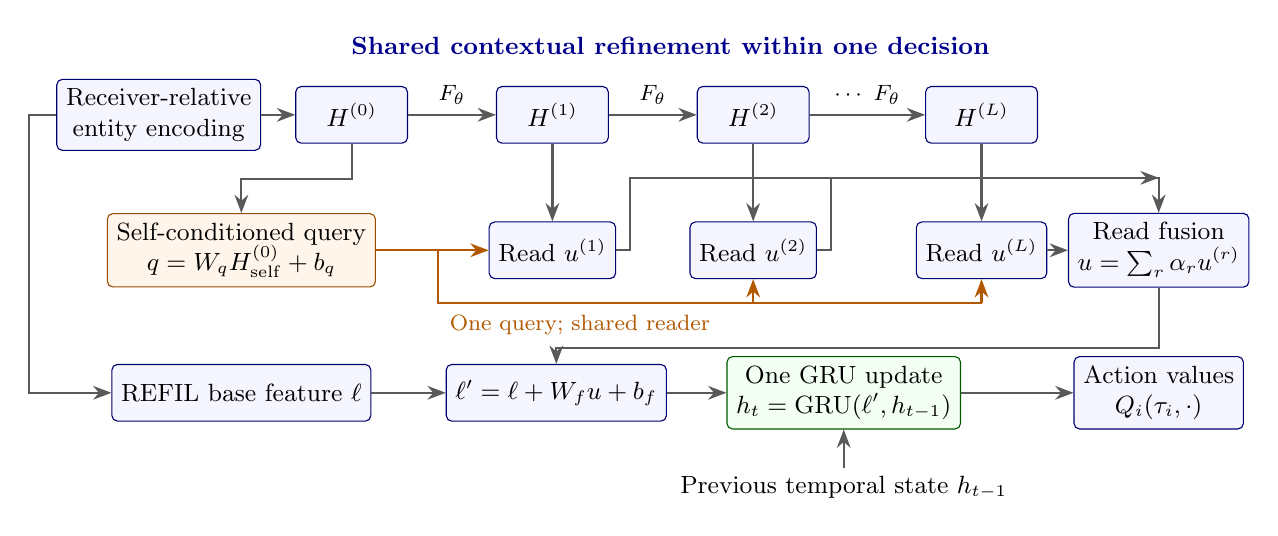
\begin{tikzpicture}[x=1cm,y=1cm,>=Stealth,
 box/.style={draw=blue!45!black,rounded corners=2pt,fill=blue!4,align=center,font=\small,minimum height=.72cm},
 smallbox/.style={box,minimum width=1.42cm},
 flow/.style={->,thick,draw=black!65},
 every node/.style={font=\small}]
\node[box,minimum width=2.1cm] (obs) at (0,0) {Receiver-relative\\entity encoding};
\node[smallbox] (h0) at (2.45,0) {$H^{(0)}$};
\node[smallbox] (h1) at (5.00,0) {$H^{(1)}$};
\node[smallbox] (h2) at (7.55,0) {$H^{(2)}$};
\node[smallbox] (hl) at (10.45,0) {$H^{(L)}$};
\draw[flow] (obs) -- (h0);
\draw[flow] (h0) -- node[above,font=\footnotesize] {$F_\theta$} (h1);
\draw[flow] (h1) -- node[above,font=\footnotesize] {$F_\theta$} (h2);
\draw[flow] (h2) -- node[above,font=\footnotesize] {$\cdots\ F_\theta$} (hl);
\node[font=\small\bfseries,text=blue!55!black] at (6.5,.88) {Shared contextual refinement within one decision};
\node[box,fill=orange!8,draw=orange!60!black,minimum width=2.1cm] (query) at (1.05,-1.72) {Self-conditioned query\\$q=W_q H^{(0)}_{\mathrm{self}}+b_q$};
\node[smallbox] (u1) at (5,-1.72) {Read $u^{(1)}$};
\node[smallbox] (u2) at (7.55,-1.72) {Read $u^{(2)}$};
\node[smallbox] (ul) at (10.45,-1.72) {Read $u^{(L)}$};
\draw[flow] (h0.south) -- ++(0,-.45) -| (query.north);
\draw[flow] (h1) -- (u1);
\draw[flow] (h2) -- (u2);
\draw[flow] (hl) -- (ul);
\draw[flow,draw=orange!70!black] (query.east) -- (u1.west);
\draw[draw=orange!70!black,thick] (3.55,-1.72) -- (3.55,-2.39) -- (10.45,-2.39);
\draw[flow,draw=orange!70!black] (7.55,-2.39) -- (u2.south);
\draw[flow,draw=orange!70!black] (10.45,-2.39) -- (ul.south);
\node[font=\footnotesize,text=orange!70!black] at (5.35,-2.67) {One query; shared reader};
\node[box,minimum width=2.05cm] (fusion) at (12.70,-1.72) {Read fusion\\$u=\sum_r\alpha_r u^{(r)}$};
\draw[flow] (ul) -- (fusion);
\draw[flow] (u1.east) -- ++(.18,0) |- (12.7,-.8) -- (fusion.north);
\draw[flow] (u2.east) -- ++(.18,0) |- (12.7,-.8);
\node[box,minimum width=2.5cm] (base) at (1.05,-3.53) {REFIL base feature $\ell$};
\node[box,minimum width=2.0cm] (res) at (5.05,-3.53) {$\ell'=\ell+W_f u+b_f$};
\node[box,fill=green!5,draw=green!35!black,minimum width=2cm] (gru) at (8.7,-3.53) {One GRU update\\$h_t=\operatorname{GRU}(\ell',h_{t-1})$};
\node[box,minimum width=1.8cm] (qval) at (12.7,-3.53) {Action values\\$Q_i(\tau_i,\cdot)$};
\draw[flow] (obs.west) -- (-1.65,0) |- (base.west);
\draw[flow] (base) -- (res);
\draw[flow] (fusion.south) -- ++(0,-.18) |- (5.05,-2.96) -- (res.north);
\draw[flow] (res) -- (gru);
\draw[flow] (gru) -- (qval);
\node at (8.7,-4.73) {Previous temporal state $h_{t-1}$};
\draw[flow] (8.7,-4.48) -- (gru.south);
\end{tikzpicture}
}
\caption{LEAF at one defender decision. A shared contextual-update block processes the receiver-relative entities for $L$ rounds. The defender's self-state query reads each intermediate representation, and learned fusion combines the resulting summaries. The fused read augments the REFIL feature before one GRU update. The loop processes the current observation; the GRU carries memory between observations. Training samples $L\in\{1,2,3,4\}$ and formal evaluation uses $L=4$.}
\label{fig:framework}
\end{figure*}
\section{Looped Entity Attention Fusion}
\label{sec:method}
LEAF constructs a decision feature in two steps: it develops context among the observed entities and reads that context for the acting defender. A shared loop and an intermediate-read fusion implement these steps jointly. The fused feature enters a recurrent utility network, which maintains the defender's history across physical decisions. Figure~\ref{fig:framework} shows the information flow.

\subsection{Receiver-Relative Entity Encoding}
At physical time $t$, defender $i$ receives the entity matrix $X_{i,t}$. Other entities are expressed relative to this defender, while the self row retains its absolute features. Inputs include normalized positions and velocities, entity type, health or alive status, target damage, and previous actions. Let $m_{i,t,e}\in\{0,1\}$ indicate whether entity $e$ is a permitted key. The main branch uses the observed entities; REFIL's imagined branches additionally apply their partition masks.

A shared encoder produces entity embeddings $e_{i,t,e}$ and the REFIL feature $\ell_{i,t}$. The initial relational representation has width $d=64$:
\begin{equation}
 H^{(0)}_{i,t,e}=W_g e_{i,t,e}+b_g.
 \label{eq:workspace}
\end{equation}
The self token supplies the receiver's query, and the mask determines the entities participating in contextual updates and reading. All defenders use the same parameters. A new observation initializes a new entity representation, so changing population size changes the input set while preserving the encoder and action interface.

\subsection{Shared Refinement and Intermediate Reading}
Suppressing defender and time indices, one contextual update is
\begin{align}
 J^{(r)}&=\operatorname{LN}_a(H^{(r-1)}),\nonumber\\
 \widetilde H^{(r)}&=H^{(r-1)}+
       \operatorname{MHA}_{\theta}(J^{(r)},H^{(r-1)},H^{(r-1)};m),\nonumber\\
 H^{(r)}&=\operatorname{Mask}_{m}\!\left[\widetilde H^{(r)}+
       \operatorname{FFN}_{\theta}(\operatorname{LN}_f(\widetilde H^{(r)}))\right].
 \label{eq:loop}
\end{align}
Here $\operatorname{LN}$ is rowwise layer normalization, $\operatorname{MHA}(Q,K,V;m)$ is masked multihead attention, and $\operatorname{Mask}_m$ zeros excluded rows. The feedforward layer has hidden width $2d$. The same parameters $\theta$ are used for all $L$ rounds. Every permitted entity can interact in the first round; subsequent rounds update features that already contain entity context. For example, an attacker's representation can be processed together with representations of the defenders and targets around it. The shared operator learns this contextual transformation across processing depths~\cite{zambaldi2019relational,dehghani2019universal}.

The acting defender reads each intermediate representation with one query derived from its initial self token:
\begin{align}
 q_{i,t}&=W_q H^{(0)}_{i,t,\mathrm{self}}+b_q,\nonumber\\
 u_{i,t}^{(r)}&=\operatorname{MHA}_{\mathrm{read}}
          (q_{i,t},H_{i,t}^{(r)},H_{i,t}^{(r)};m_{i,t}).
 \label{eq:read}
\end{align}
The query and reader parameters are shared across rounds at a decision. This produces a sequence of defender-specific summaries $u_{i,t}^{(1)},\ldots,u_{i,t}^{(L)}$. The loop supplies the entity context; the query determines how the receiver accesses it.

A scalar scoring map combines these summaries:
\begin{equation}
 \alpha_{i,t}^{(r)}=
 \frac{\exp(w_s^\top u_{i,t}^{(r)}+b_s)}
 {\sum_{j=1}^{L}\exp(w_s^\top u_{i,t}^{(j)}+b_s)},\qquad
 u_{i,t}=\sum_{r=1}^{L}\alpha_{i,t}^{(r)}u_{i,t}^{(r)}.
 \label{eq:fusion}
\end{equation}
Entity attention selects information within a processing stage; fusion combines information across stages. The weights are computed from the receiver-specific reads at each decision. Preserving these reads gives the controller direct access to intermediate context~\cite{xu2018jk}. All $L$ rounds are executed, and fusion determines their contribution to the final feature.

\subsection{Recurrent Cooperative Decision}
The relational read augments the REFIL feature through a residual projection:
\begin{align}
 \ell'_{i,t}&=\ell_{i,t}+W_f u_{i,t}+b_f,\nonumber\\
 h_{i,t}&=\operatorname{GRU}(\ell'_{i,t},h_{i,t-1}),\nonumber\\
 Q_i(\tau_{i,t},\cdot)&=W_o h_{i,t}+b_o.
 \label{eq:decision}
\end{align}
The residual projection is initialized to zero; both feature paths are then learned jointly. The GRU updates once per physical decision and carries its hidden state to the next observation. Thus processing round $r$ develops current entity context, while physical time $t$ advances the temporal state. This placement lets the reader use the current defender state and lets the decision network combine that read with its motion history. Decentralized execution selects the legal action with highest utility.

The trained memory-query comparison adds the preceding GRU state to Eq.~\eqref{eq:read}, with the gradient stopped through that query input. Both designs retain the recurrent decision network. The comparison therefore examines the location of temporal information within the encoder.

\subsection{Training and Population Transfer}
Collection samples $L$ uniformly from $\{1,2,3,4\}$ and holds it fixed for an episode. Replay independently samples one depth per minibatch for the online main and imagined branches and the target network. The shared block is consequently trained both as a short contextual transform and as an operator on its own preceding outputs. Formal evaluation fixes $L=4$.

Training retains the host's potential-shaped reward,
\begin{align}
 \widetilde r_t&=-\Delta D_t+\gamma\Phi(s_{t+1})-\Phi(s_t),\nonumber\\
 \Phi(s)&=-\sum_{j\in\mathcal B_{\mathrm{alive}}}
 \operatorname{clip}\!\left(1-\frac{\min_{k\in\mathcal T}\|p_j-p_k\|}{4000},0,1\right),
 \label{eq:shaping}
\end{align}
where $p_j$ and $p_k$ are attacker and target positions and $\gamma=0.99$. This potential provides a dense proximity signal. Evaluation uses the unshaped reward $R=-D$.

Let $\bar r_t$ denote the replay reward and $b_t$ the bootstrap multiplier. Natural termination uses $b_t=0$; ordinary transitions use $b_t=\gamma$, and time-limit transitions retain a successor. If the final defender disappears, the discounted reward tail from the remaining simulation is included in its final decision transition. Online utilities select the legal greedy successor actions $\boldsymbol a^*_{t+1}$, giving the target
\begin{equation}
 y_t=\bar r_t+b_t Q^-_{\mathrm{tot}}(x_{t+1},\boldsymbol a^*_{t+1}).
 \label{eq:td-target}
\end{equation}
The main and imagined values are trained against this target:
\begin{align}
 \mathcal L&=(1-\lambda)\mathcal L_{\mathrm{main}}
                  +\lambda\mathcal L_{\mathrm{aux}},\qquad\lambda=0.5,\nonumber\\
 \mathcal L_k&=\frac{\sum_{b,t} v_{b,t}(Q_{k,b,t}-y_{b,t})^2}
 {\sum_{b,t}v_{b,t}},\quad k\in\{\mathrm{main},\mathrm{aux}\},
 \label{eq:td-loss}
\end{align}
where $v_{b,t}$ marks valid replay transitions and the target is detached during optimization. Both branches share parameters and reconstruct their masked histories. Deployment uses the main branch, as summarized in Algorithm~\ref{alg:leaf}.

\begin{algorithm}[!t]
\caption{LEAF at one defender decision}
\label{alg:leaf}
\begin{algorithmic}[1]
\Require Entities $X_{i,t}$, mask $m_{i,t}$, memory $h_{i,t-1}$, depth $L$
\State Encode entities and compute base feature $\ell_{i,t}$
\State Initialize $H^{(0)}_{i,t}$ and query $q_{i,t}$
\For{$r=1,\ldots,L$}
\State Update $H^{(r)}_{i,t}$ with shared block, Eq.~\eqref{eq:loop}
\State Read $u^{(r)}_{i,t}$ with $q_{i,t}$, Eq.~\eqref{eq:read}
\EndFor
\State Fuse reads and augment $\ell_{i,t}$, Eqs.~\eqref{eq:fusion}--\eqref{eq:decision}
\State Update temporal state and compute action values
\State \Return $\arg\max_{a\in\mathcal U_{i,t}}Q_i(\tau_{i,t},a)$ and $h_{i,t}$
\end{algorithmic}
\end{algorithm}

Shared rowwise maps and masked attention make the encoder consistent with entity ordering: permuting non-self entities and their masks permutes the intermediate representations and preserves the receiver's read and action values. Parameter count is independent of entity count and unfolding depth. For $M$ entity slots and width $d$, the relational updates cost $O(L(M^2d+Md^2))$ per receiver. The same controller can therefore accept different populations through its entity set and mask; Section~\ref{sec:results} evaluates the resulting protection performance.

\section{Experimental Evaluation}
\label{sec:results}
% Numerical source: ../data/paper1007.json; no scientific statistics recomputed.
% Display names map existing saved designs; SD unit is stated in each caption.

\newcommand{\HadMainTable}{%
\begin{table*}[!t]
\centering\footnotesize
\setlength{\tabcolsep}{5pt}
\caption{Formal comparison: mean $\pm$ sample SD. Reward $R=-D$ is higher-is-better; friendly-collision mortality $C$ is lower-is-better. Each learned method has three training seeds and 300 common scenes per configuration. Bold marks the best group mean for each metric.}
\label{tab:had-main}
\begin{tabular*}{\textwidth}{@{\extracolsep{\fill}}llrrrr@{}}
\toprule
Method & Metric & ID & $K$-OOD & $N$-OOD & Joint OOD \\
\midrule
\textbf{LEAF} & $R\uparrow$ & $\mathbf{-0.405\pm0.097}$ & $\mathbf{-0.996\pm0.233}$ & $\mathbf{-0.575\pm0.235}$ & $\mathbf{-1.097\pm0.105}$ \\
 & $C\downarrow$ (\%) & $\mathbf{1.33\pm0.45}$ & $\mathbf{1.70\pm0.62}$ & $6.29\pm1.32$ & $4.97\pm1.26$ \\
\addlinespace[2pt]
REFIL & $R\uparrow$ & $-0.715\pm0.049$ & $-1.796\pm0.304$ & $-2.209\pm0.277$ & $-3.308\pm0.303$ \\
 & $C\downarrow$ (\%) & $2.97\pm0.42$ & $4.71\pm0.67$ & $12.86\pm2.14$ & $10.34\pm1.69$ \\
\addlinespace[2pt]
QMIX-Atten & $R\uparrow$ & $-2.318\pm1.431$ & $-5.009\pm2.497$ & $-5.139\pm3.111$ & $-7.415\pm3.970$ \\
 & $C\downarrow$ (\%) & $10.82\pm9.56$ & $12.42\pm9.75$ & $16.38\pm5.43$ & $15.37\pm7.34$ \\
\addlinespace[2pt]
DCG & $R\uparrow$ & $-2.028\pm0.437$ & $-5.839\pm1.920$ & $-5.021\pm2.658$ & $-8.092\pm3.909$ \\
 & $C\downarrow$ (\%) & $9.05\pm3.36$ & $14.97\pm4.68$ & $19.70\pm8.52$ & $19.26\pm10.20$ \\
\addlinespace[2pt]
SPECTra & $R\uparrow$ & $-2.662\pm0.070$ & $-6.933\pm0.670$ & $-6.455\pm1.403$ & $-11.184\pm0.352$ \\
 & $C\downarrow$ (\%) & $13.06\pm0.75$ & $20.71\pm1.60$ & $28.92\pm1.54$ & $31.25\pm1.63$ \\
\addlinespace[2pt]
ALMA & $R\uparrow$ & $-1.326\pm0.193$ & $-3.022\pm0.344$ & $-3.605\pm0.742$ & $-5.375\pm1.036$ \\
 & $C\downarrow$ (\%) & $7.42\pm1.13$ & $9.05\pm1.66$ & $18.42\pm3.84$ & $15.92\pm3.86$ \\
\addlinespace[2pt]
Rule$^{\dagger}$ & $R\uparrow$ & $-1.462\pm0.717$ & $-3.212\pm1.126$ & $-1.545\pm0.881$ & $-3.060\pm0.976$ \\
 & $C\downarrow$ (\%) & $1.98\pm4.47$ & $2.70\pm3.57$ & $\mathbf{5.70\pm3.30}$ & $\mathbf{4.48\pm2.44}$ \\
\bottomrule
\end{tabular*}
\par\vspace{2pt}\parbox{\textwidth}{\footnotesize
$\dagger$ Rule has no training seeds. Its SD is across the 300 scene seeds, after averaging configurations within each scene. All other SDs measure training-seed variation. Collision SDs are percentage points.}
\end{table*}}

\newcommand{\HadCoreAblationTable}{%
\begin{table*}[!t]
\centering\footnotesize
\setlength{\tabcolsep}{5pt}
\caption{Trained design comparisons: absolute reward $R=-D$ and friendly-collision mortality $C$, mean $\pm$ sample SD across three training seeds. Each configuration uses 300 common scenes. Bold marks the best mean among these five designs.}
\label{tab:had-core-ablation}
\begin{tabular*}{\textwidth}{@{\extracolsep{\fill}}llrrrr@{}}
\toprule
Method & Metric & ID & $K$-OOD & $N$-OOD & Joint OOD \\
\midrule
\textbf{LEAF} & $R\uparrow$ & $\mathbf{-0.405\pm0.097}$ & $\mathbf{-0.996\pm0.233}$ & $\mathbf{-0.575\pm0.235}$ & $\mathbf{-1.097\pm0.105}$ \\
 & $C\downarrow$ (\%) & $\mathbf{1.33\pm0.45}$ & $\mathbf{1.70\pm0.62}$ & $\mathbf{6.29\pm1.32}$ & $\mathbf{4.97\pm1.26}$ \\
\addlinespace[2pt]
Memory query & $R\uparrow$ & $-0.527\pm0.227$ & $-1.529\pm0.734$ & $-0.998\pm0.621$ & $-1.946\pm1.229$ \\
 & $C\downarrow$ (\%) & $1.66\pm0.86$ & $2.59\pm1.78$ & $8.57\pm4.41$ & $6.65\pm4.16$ \\
\addlinespace[2pt]
No host & $R\uparrow$ & $-0.510\pm0.138$ & $-1.768\pm0.621$ & $-1.263\pm0.653$ & $-2.319\pm0.889$ \\
 & $C\downarrow$ (\%) & $2.23\pm0.77$ & $3.67\pm1.65$ & $10.71\pm3.98$ & $8.76\pm3.14$ \\
\addlinespace[2pt]
Direct read & $R\uparrow$ & $-0.928\pm0.210$ & $-1.958\pm0.457$ & $-2.020\pm0.446$ & $-3.196\pm0.687$ \\
 & $C\downarrow$ (\%) & $3.34\pm1.66$ & $4.46\pm2.10$ & $11.16\pm1.81$ & $9.17\pm2.18$ \\
\addlinespace[2pt]
One round & $R\uparrow$ & $-0.609\pm0.272$ & $-1.203\pm0.402$ & $-1.355\pm0.884$ & $-2.157\pm1.006$ \\
 & $C\downarrow$ (\%) & $1.57\pm0.15$ & $2.08\pm0.32$ & $8.35\pm3.16$ & $6.56\pm2.37$ \\
\bottomrule
\end{tabular*}
\par\vspace{2pt}\parbox{\textwidth}{\footnotesize
Configurations are weighted equally within each training seed. Memory query adds incoming GRU history to LEAF's reader query. No host removes the local host, imagination, and associated losses from the memory-query design. Direct read and One round retain query history and execute zero and one contextual update, respectively. Collision SDs are percentage points.}
\end{table*}}

\newcommand{\HadFullVariantTable}{%
\begin{table*}[!t]
\centering\footnotesize
\setlength{\tabcolsep}{5pt}
\caption{All ten completed trained designs: reward mean $\pm$ sample SD across three training seeds on the same formal matrix. Bold marks the best group mean. All designs share the evaluation configurations.}
\label{tab:had-full-variants}
\begin{tabular*}{\textwidth}{@{\extracolsep{\fill}}lrrrr@{}}
\toprule
Method & ID & $K$-OOD & $N$-OOD & Joint OOD \\
\midrule
\textbf{LEAF} & $\mathbf{-0.405\pm0.097}$ & $\mathbf{-0.996\pm0.233}$ & $-0.575\pm0.235$ & $\mathbf{-1.097\pm0.105}$ \\
Memory query & $-0.527\pm0.227$ & $-1.529\pm0.734$ & $-0.998\pm0.621$ & $-1.946\pm1.229$ \\
No host & $-0.510\pm0.138$ & $-1.768\pm0.621$ & $-1.263\pm0.653$ & $-2.319\pm0.889$ \\
Direct read & $-0.928\pm0.210$ & $-1.958\pm0.457$ & $-2.020\pm0.446$ & $-3.196\pm0.687$ \\
One round & $-0.609\pm0.272$ & $-1.203\pm0.402$ & $-1.355\pm0.884$ & $-2.157\pm1.006$ \\
Last read & $-0.434\pm0.083$ & $-1.020\pm0.100$ & $-0.652\pm0.160$ & $-1.269\pm0.202$ \\
Fixed depth & $-0.407\pm0.204$ & $-1.004\pm0.665$ & $-0.659\pm0.184$ & $-1.265\pm0.230$ \\
Initial keys & $-0.469\pm0.091$ & $-1.221\pm0.344$ & $-1.778\pm1.292$ & $-2.370\pm1.164$ \\
Unshared rounds & $-0.476\pm0.183$ & $-1.127\pm0.157$ & $\mathbf{-0.543\pm0.156}$ & $-1.232\pm0.253$ \\
Count inputs & $-0.596\pm0.145$ & $-1.301\pm0.427$ & $-1.075\pm0.449$ & $-1.685\pm0.844$ \\
\bottomrule
\end{tabular*}
\par\vspace{2pt}\parbox{\textwidth}{\footnotesize
The five core names follow Table~\ref{tab:had-core-ablation}. Last read uses only the final read; Fixed depth trains and executes four rounds; Initial keys anchors keys and values to the initial entity set; Unshared rounds trains four independent update blocks; Count inputs adds typed-count features. These five designs also retain query history. Unshared rounds is compared with Fixed depth to separate sharing under a matched depth schedule.}
\end{table*}}

\newcommand{\HadCapacityTable}{%
\begin{table*}[!t]
\centering\footnotesize
\setlength{\tabcolsep}{5pt}
\caption{Capacity reference: reward and friendly-collision mortality, mean $\pm$ sample SD across three training seeds. The enlarged REFIL reference approximately matches LEAF's actor parameter budget; all methods use the same formal evaluation scenes.}
\label{tab:had-capacity}
\begin{tabular*}{\textwidth}{@{\extracolsep{\fill}}llrrrr@{}}
\toprule
Method & Metric & ID & $K$-OOD & $N$-OOD & Joint OOD \\
\midrule
\textbf{LEAF} & $R\uparrow$ & $\mathbf{-0.405\pm0.097}$ & $\mathbf{-0.996\pm0.233}$ & $\mathbf{-0.575\pm0.235}$ & $\mathbf{-1.097\pm0.105}$ \\
 & $C\downarrow$ (\%) & $\mathbf{1.33\pm0.45}$ & $\mathbf{1.70\pm0.62}$ & $\mathbf{6.29\pm1.32}$ & $\mathbf{4.97\pm1.26}$ \\
\addlinespace[2pt]
REFIL & $R\uparrow$ & $-0.715\pm0.049$ & $-1.796\pm0.304$ & $-2.209\pm0.277$ & $-3.308\pm0.303$ \\
 & $C\downarrow$ (\%) & $2.97\pm0.42$ & $4.71\pm0.67$ & $12.86\pm2.14$ & $10.34\pm1.69$ \\
\addlinespace[2pt]
REFIL (matched) & $R\uparrow$ & $-0.914\pm0.165$ & $-2.493\pm0.280$ & $-2.269\pm0.312$ & $-4.170\pm0.760$ \\
 & $C\downarrow$ (\%) & $4.12\pm0.46$ & $6.86\pm2.30$ & $12.40\pm3.09$ & $12.02\pm4.17$ \\
\bottomrule
\end{tabular*}
\par\vspace{2pt}\parbox{\textwidth}{\footnotesize
Actor parameter counts are 175,754 for LEAF, 102,025 for REFIL, and 176,393 for REFIL (matched). Collision SDs are percentage points.}
\end{table*}}


\noindent\textbf{Setup.}
We evaluate target protection in the planar model of SkyHAD 3.0.0~\cite{skyhad2026}, with public entity-state observations, a fixed reactive--rush attacker, and a horizon of 100 physical steps. Training samples balanced teams $N_R=N_B=N\in\{4,6,8,10\}$ and target counts $K\in\{1,2,3\}$. Each learned method uses three training seeds and a budget of $10^6$ physical environment steps per seed. LEAF has hidden width 64, four attention heads, learning rate $5\times10^{-4}$, discount 0.99, batch size 32, and replay capacity 5000. Training samples one to four relational rounds; formal evaluation uses four.

Final policies execute with frozen parameters on 24 configurations, each with 300 common initial scenes. In-distribution (ID) configurations are $(4,4,2)$, $(6,6,2)$, $(8,8,2)$, and $(10,10,3)$, written as $(N_R,N_B,K)$. Target-count extrapolation ($K$-OOD) uses $(10,10,K)$ for $K\in\{4,6,9,12\}$; team-size extrapolation ($N$-OOD) uses $(N,N,2)$ for $N\in\{15,20,25,30,40,50\}$. Joint extrapolation combines $N\in\{15,20,30\}$ with $K\in\{4,6\}$ and includes $(30,30,9)$ and $(30,30,12)$. The remaining configurations, $(5,5,2)$ and $(10,10,2)$, provide intermediate-scale reference points. The five learned baselines are REFIL~\cite{iqbal2021refil}, QMIX with an entity-attention encoder (QMIX-Atten)~\cite{rashid2018qmix}, DCG~\cite{boehmer2020dcg}, SPECTra~\cite{park2026spectra}, and ALMA~\cite{iqbal2022alma}. Rule provides a fixed-controller reference.

\noindent\textbf{Metrics and aggregation.}
The primary metric is episode reward $R=-D$, with higher values indicating better target protection. Friendly-collision mortality,
\begin{equation}
 C=\frac{\text{defenders killed by friendly collision}}{N_R},
\end{equation}
measures losses within the protecting team. Each model first averages the 300 scenes within a configuration and then averages configurations equally within a group. Tables report mean $\pm$ sample standard deviation (SD) across the three trained models~\cite{agarwal2021rliable}. For Rule, the reported SD is across 300 scene seeds after averaging configurations within each seed.

Learning curves use 50 validation checkpoints. Each checkpoint evaluates four ID configurations with 25 fixed scenes each, separate from the formal evaluation scenes. We align validation indices across training seeds and plot the mean reward at the mean recorded environment-step count. Bands show the three-model sample SD, without smoothing.

\subsection{Comparison Across Deployment Populations}
\label{subsec:comparison}
LEAF obtains the highest group mean reward among the six learned methods and Rule in all four groups (Table~\ref{tab:had-main}). Relative to REFIL, the reward gains are 0.310, 0.800, 1.635, and 2.211 for ID, $K$-OOD, $N$-OOD, and Joint OOD, respectively. All three corresponding training-seed comparisons favor LEAF in each group. The larger gains under team-size and joint extrapolation show the value of the relational encoder when a defender must coordinate within a larger entity set.

Figure~\ref{fig:had-generalization} connects learning to deployment. At the tenth validation checkpoint, approximately $0.2$ million environment steps, LEAF reaches $-2.046\pm0.028$ compared with REFIL's $-4.429\pm0.284$. At the final checkpoint, the rewards are $-0.373\pm0.066$ and $-0.738\pm0.122$. The other panels follow the frozen policies as target count, team size, and both populations increase. Presenting each joint configuration separately preserves the distinct changes in threats and assets.

LEAF also has lower mean friendly-collision mortality than each learned baseline in all four groups. Rule incurs fewer collision deaths in $N$-OOD and Joint OOD, at 5.70\% and 4.48\%, compared with LEAF's 6.29\% and 4.97\%. Its corresponding rewards are lower. The two metrics therefore distinguish conserving defenders from protecting the targets: LEAF combines low friendly losses with more effective defense.

\HadMainTable

\begin{figure*}[!t]
\centering
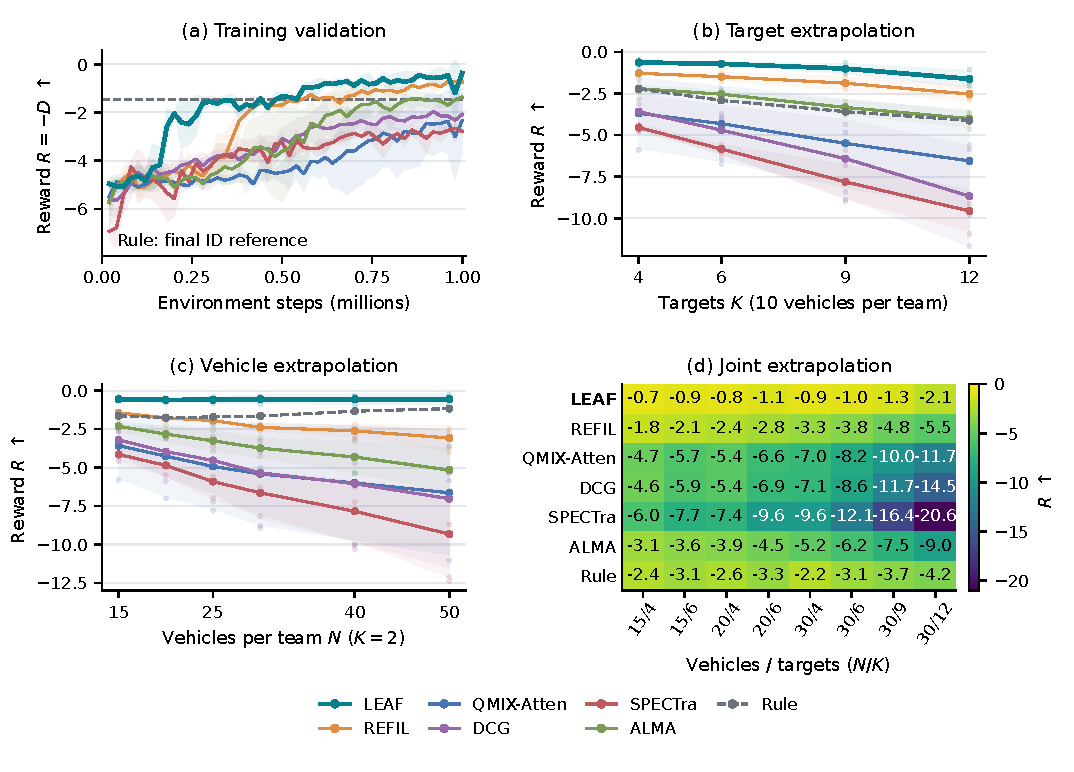
\includegraphics[width=\textwidth]{figures/fig_had_generalization.pdf}
\caption{Learning and population transfer. (a) Fifty validation checkpoints for LEAF and five learned baselines at recorded environment steps; bands show one model-seed sample SD. The Rule line marks its final ID reward. (b)--(c) Frozen-policy reward under target-count and team-size extrapolation, with seed points and SD bands for learned methods. (d) Reward at the eight joint-extrapolation configurations on a common linear scale.}
\label{fig:had-generalization}
\end{figure*}

\subsection{Ablation and Design Comparisons}
\label{subsec:ablation}
The trained comparisons address three aspects of the encoder: constructing context before reading, locating temporal memory, and combining the relational feature with its host. Table~\ref{tab:had-core-ablation} and Fig.~\ref{fig:had-ablation} give both learning trajectories and population-transfer results. The \emph{Memory query} design adds detached previous GRU state to the reader query. \emph{Direct read}, \emph{One round}, and \emph{No host} use this same memory-query formulation, providing the paired design comparisons below.

\noindent\textbf{Context before reading.}
Direct read applies the reader to the initial entity representations. One round performs one shared contextual update before reading. The latter improves group mean reward by 0.319, 0.755, 0.665, and 1.039 in ID, $K$-OOD, $N$-OOD, and Joint OOD, with two of three seed pairs improving in each group. The consistent direction across population groups supports processing entity relationships before compressing them into the defender's decision feature.

\noindent\textbf{Current-state reading with downstream memory.}
Memory query and LEAF both preserve the recurrent decision network. Using only the current self state for the query gives LEAF mean reward gains of 0.122, 0.533, 0.424, and 0.849 across the four groups. The gains hold for three seeds in ID and two seeds in each extrapolation group. The result favors the chosen division of computation: the reader extracts the current relational context, and the downstream GRU combines it with temporal history.

\noindent\textbf{Integration with cooperative value learning.}
No host retains the relational path while removing the REFIL feature path, imagined branches, and associated auxiliary loss. Restoring this host in the Memory query design improves the three extrapolation-group rewards by 0.239, 0.265, and 0.372; the ID mean changes by $-0.017$. LEAF then combines the retained host with current-state reading. Although No host reaches a final ID validation reward of $-0.381\pm0.126$, close to LEAF's $-0.373\pm0.066$, their transfer results differ substantially. This contrast shows why the evaluation must examine deployment populations alongside training validation.

\HadCoreAblationTable

\begin{figure*}[!t]
\centering
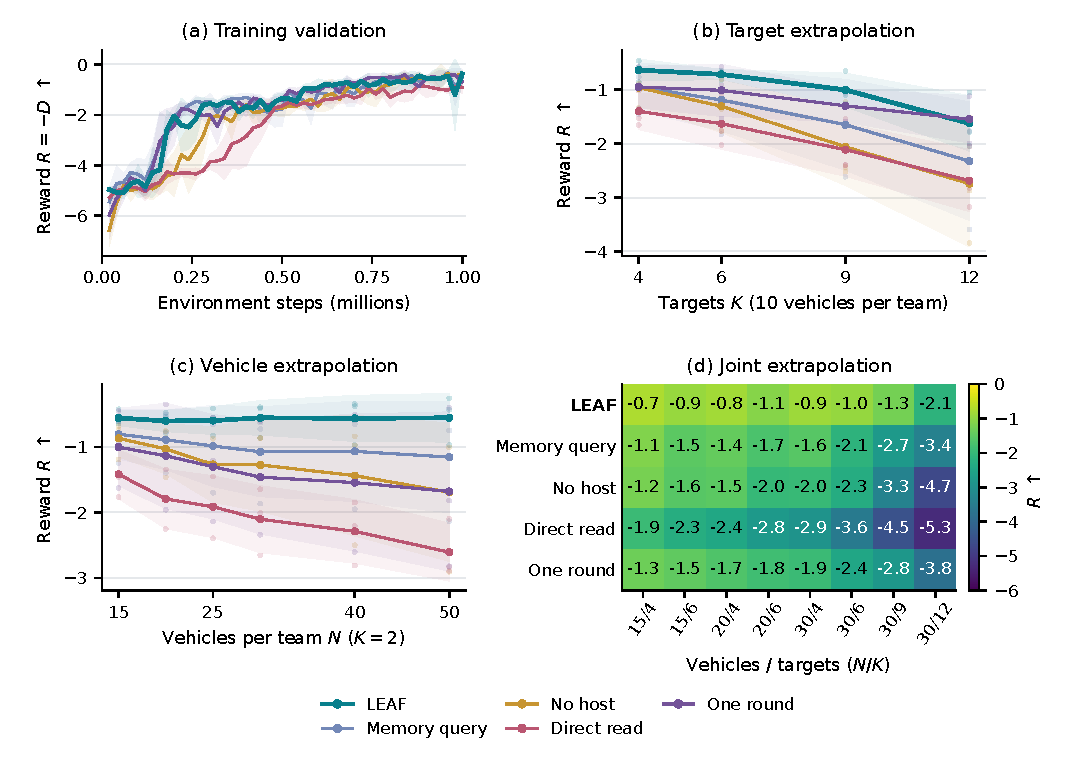
\includegraphics[width=\textwidth]{figures/fig_had_ablation.pdf}
\caption{Trained design comparisons. (a) Validation reward over 50 checkpoints; lines and bands show the three-model mean and sample SD at actual mean environment steps. (b)--(c) Target-count and team-size extrapolation. (d) Joint-extrapolation rewards on a common linear scale. Memory query adds temporal state to LEAF's reader. Direct read, One round, and No host use that memory-query formulation; their paired comparisons are described in the text.}
\label{fig:had-ablation}
\end{figure*}

A parameter-matched REFIL control has 176,393 actor parameters, close to LEAF's 175,754; standard REFIL has 102,025. Its group rewards are $-0.914\pm0.165$, $-2.493\pm0.280$, $-2.269\pm0.312$, and $-4.170\pm0.760$. LEAF exceeds this control in all three seed comparisons for every group. The performance gain thus persists when the host is given a comparable parameter budget.

\subsection{Mechanism of Relational Encoding}
\label{subsec:mechanism}
The mechanism study follows the computation introduced in Section~\ref{sec:method}: contextual updates produce intermediate entity sets, the self-conditioned reader combines them into a decision feature, and the resulting actions determine interception and protection. We examine execution at the depths used during training, record the normal intermediate reads, and relate the policy's outcome to the formal protection metrics.

\noindent\textbf{Protection across processing depths.}
We execute each frozen LEAF model at $L\in\{1,2,3,4\}$ on ten common scenes in each of three configurations: $(10,10,2)$, $(30,30,2)$, and $(30,30,12)$. The first two vary team size at fixed target count; the last two vary target count at fixed team size. All four paths use the trained update block, reader, fusion, and recurrent decision network. REFIL runs on the same scenes. Reward is averaged over scenes within each model and then reported across three model seeds; differences between depths are paired by model and scene.

Figure~\ref{fig:leaf-depth} shows that all four LEAF depths have higher mean reward than REFIL in these three configurations. At 10v10 and 30v30 with two targets, two-round execution has paired reward differences of $-0.273\pm0.047$ and $-0.363\pm0.291$ relative to four rounds, with all three model means lower. Three and four rounds give the same reward at 10v10; three rounds give $0.146\pm0.131$ higher reward at 30v30 with two targets and $0.793\pm0.907$ lower reward with twelve targets. Thus the ordering of execution depths changes with the engagement. Together with the trained Direct read--One round comparison, these results locate the common advantage in useful contextual representations, with later processing altering protection according to the scene.

\begin{figure*}[!t]
\centering
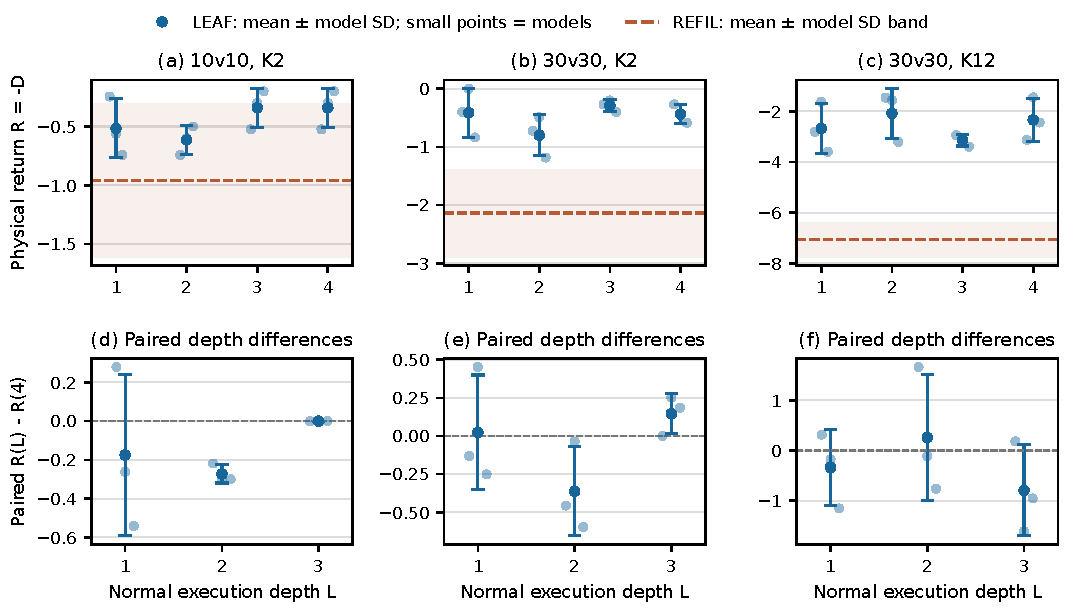
\includegraphics[width=\textwidth]{figures/fig_leaf_depth.pdf}
\caption{Frozen LEAF execution at depths used during training. Top: reward at each depth and the REFIL reference. Bottom: scene-paired reward difference from four-round execution; positive values favor the shorter path. Each point and error bar is the mean and sample SD of three model means, each based on ten scenes. Small points show individual models.}
\label{fig:leaf-depth}
\end{figure*}

\noindent\textbf{Intermediate reading varies with the defender and time.}
We record all four read vectors and fusion weights during the normal four-round executions: 90 episodes containing 38,693 live-defender decisions. Figure~\ref{fig:leaf-readout}(a) shows a clear preference for early context. The first read receives 73.66--75.65\% of mean fusion weight across the three configurations, and the first two together receive approximately 99\%. The encoder therefore supplies its recurrent policy primarily with the early contextual reads even when it executes all four updates.

The same average preference encompasses different choices by individual defenders. For the first-round weight, the within-state SD across active defenders averages 11.44, 13.91, and 12.68 percentage points in the three configurations. Tracking the same defender across adjacent physical steps gives mean absolute weight changes of 5.49, 5.34, and 5.36 percentage points. These measurements directly characterize the self-conditioned fusion: defenders observing the same engagement combine stages differently, and each defender changes that combination as the engagement evolves. The shared encoder consequently offers a common relational computation with receiver-specific access to its intermediate stages.

\begin{figure*}[!t]
\centering
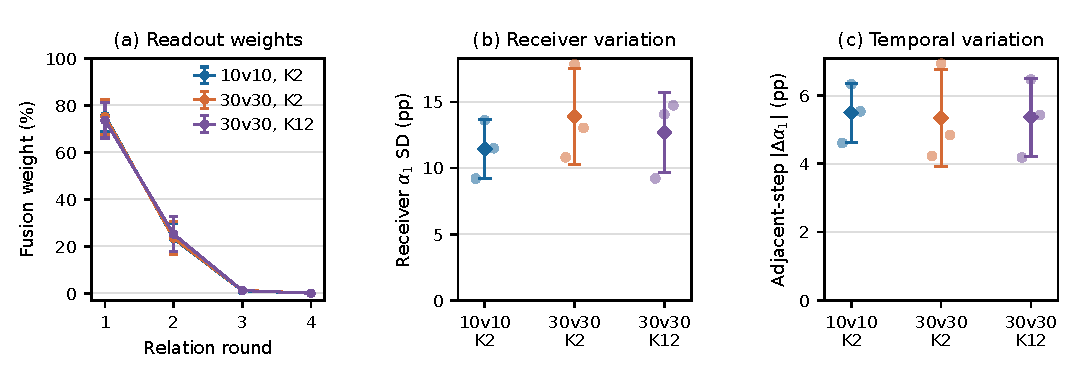
\includegraphics[width=\textwidth]{figures/fig_leaf_readout.pdf}
\caption{Intermediate-read use in normal four-round execution. (a) Mean fusion weights by round and configuration. (b) Variation among active defenders at the same physical step, measured by the population SD of the first-round weight. (c) Mean absolute change of that weight for the same defender at adjacent physical steps. Panel (b) averages over physical decision states within each model. Panel (c) averages the adjacent-step changes within each episode and then weights the ten scenes equally. Error bars show sample SD across three model means; small points retain the models in (b)--(c).}
\label{fig:leaf-readout}
\end{figure*}

\noindent\textbf{From coordinated response to target protection.}
The formal evaluation uses 300 scenes per model and configuration. Across the three mechanism configurations and the larger 50v50 case, LEAF combines higher attacker interception with lower friendly-collision mortality and less frequent target damage than REFIL. At 10v10 with two targets, interception increases from 77.00\% to 86.38\%, and target-damage incidence falls from 55.22\% to 30.44\%. At 30v30 with two targets, interception rises from 75.11\% to 83.02\% and target-damage incidence falls from 70.89\% to 29.56\%. Increasing the targets from two to twelve at the same team size preserves this direction: LEAF intercepts 81.54\% of attackers and experiences target damage in 48.33\% of episodes, compared with 74.48\% and 78.22\% for REFIL. At 50v50, LEAF retains an interception advantage of 6.41 percentage points and reduces friendly-collision mortality from 19.59\% to 11.14\%; target-damage incidence falls from 70.56\% to 28.11\%. The learned representation thus supports the intended team outcome: fewer defenders are lost to one another, more threats are intercepted, and fewer episodes allow damage to the protected assets.





\begin{figure*}[!t]
\centering
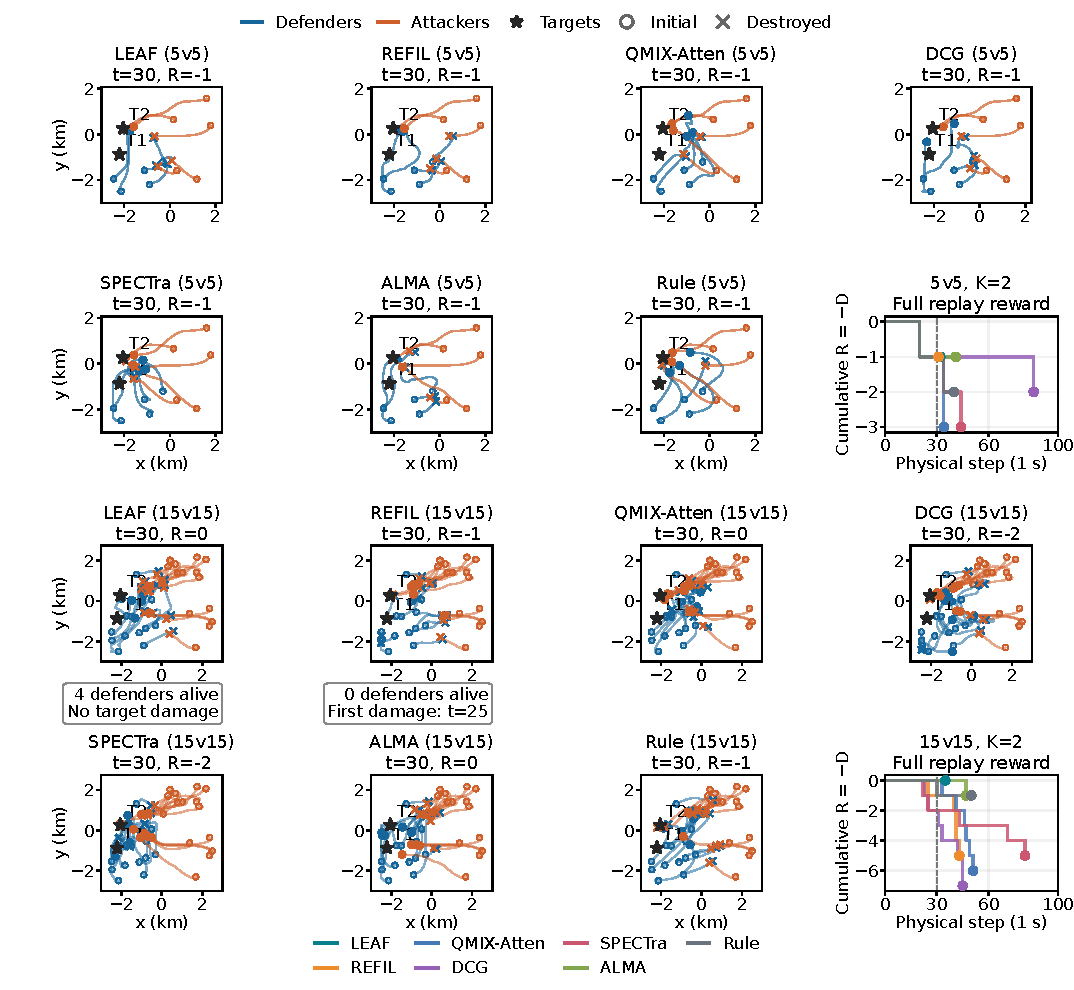
\includegraphics[width=\textwidth]{figures/fig_leaf_final1007_trajectory.pdf}
\caption{Common-scene trajectory comparison. The upper two rows show 5v5 and the lower two show 15v15, both with two targets. Each block contains seven spatial panels and a cumulative-reward plot. Paths end at the common snapshot step 30: open circles are initial positions, filled circles are live vehicles, crosses are destroyed vehicles, and stars are targets. Panel titles give reward at the snapshot. Reward curves end at the actual terminal step, marked by a dot; the dashed line marks the snapshot time. The annotations identify the two methods' defensive state at step 30 in the 15v15 case. All spatial panels within a scale share coordinates and color conventions.}
\label{fig:had-cases}
\end{figure*}

\subsection{Representative Trajectories}
\label{subsec:trajectories}
Figure~\ref{fig:had-cases} compares all seven methods at $(5,5,2)$ and $(15,15,2)$ under the same initial layout within each configuration. Learned policies use training seed 0, and both examples use scene seed 9000. Paths and entity states are shown at physical step 30; the adjacent reward curves continue to each policy's actual terminal step.

At 5v5, LEAF, REFIL, and ALMA finish with reward $-1$. LEAF and REFIL first incur target damage at step 20 and complete their engagements at steps 32 and 31. Their trajectories show different interception routes with the same final protection outcome.

The 15v15 scene exposes the effect of sustaining the defense. At the common snapshot, LEAF retains four defenders against two surviving attackers, with both targets undamaged. REFIL has lost its final defender at step 27; four attackers remain at step 30, and reward has reached $-1$. Its reward then falls to $-5$ as damage continues after the defending team disappears. LEAF intercepts all 15 attackers by step 35 and finishes with $R=0$. QMIX-Atten, DCG, SPECTra, ALMA, and Rule finish with $-6$, $-7$, $-5$, $-1$, and $-1$, respectively. The surviving-team snapshots and complete reward histories connect maintained defensive capability to the final protection outcome.



\FloatBarrier
\section{Conclusion}
LEAF uses a shared loop and self-conditioned intermediate reading to build a relational feature for cooperative target protection. The encoder develops the current entity context, combines reads from successive processing stages, and supplies the result to a recurrent utility network. This organization supports a common policy across changing numbers of defenders, attackers, and targets.

In SkyHAD, frozen LEAF policies attain higher group mean reward than five learned baselines and Rule across the four evaluated population groups. Trained comparisons favor constructing context before reading and using current-state queries with temporal memory downstream. The gains persist against a parameter-matched REFIL control. At larger populations, higher attacker interception and lower target-damage incidence connect the representation design to its intended protective outcome. The resulting controller provides an effective simulation-based approach to transferring cooperative defense policies from small training engagements to larger deployment populations.

\section*{Acknowledgment}
OpenAI Codex assisted with manuscript drafting, code-assisted analysis, and figure preparation.
\bibliographystyle{IEEEtran}
\bibliography{references}
\end{document}
